\section{Hierarchically Fused Fully Convolutional Network}
\label{Sec:HF-FCN}
In this section, we introduce our hierarchical feature fusion architecture, and apply it to the common networks, VGG16 Net and ResNet.
%
The overview diagram in Fig.~\ref{fig:Fusion-Operation} shows where the lateral connections and fusion operations take effect.
%

In order to leverage the feature pyramid while preserving fine-scale structure and high-level semantics, our network involves one bottom-up pathway for feature extraction in multiple scales, lateral connections at each individual scale, and one \fymd{tunnel} \xjmd{fusion} \cxj{another name? xx fusion?} for the final prediction.

\begin{figure}
%\vspace{-0.4cm}
%\setlength{\abovecaptionskip}{-0cm}
%\setlength{\belowcaptionskip}{-2cm}
\centering
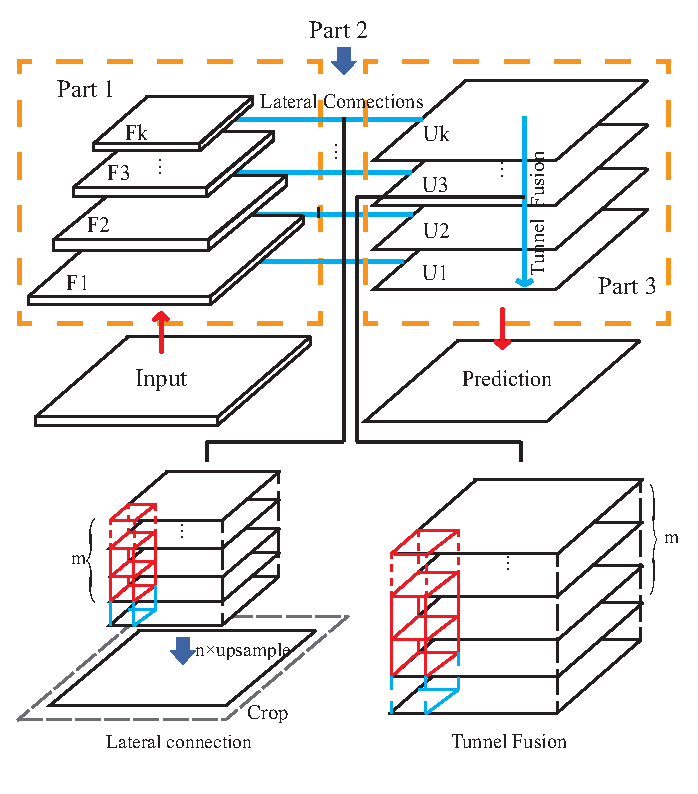
\includegraphics[width=8.5cm]{Figures/Fusion_Operation.eps}
\caption{The first line shows the overview of our network. The second row shows the details of lateral connection and tunnel fusion operation. Fk means the feature maps come from the kth layer. m for number of feature maps. n said the n times of up sampling.}
\label{fig:Fusion-Operation}
\end{figure}
%\subsection{Network Architecture}

\noindent\textbf{Bottom-up Feature Extraction.} The first part is a bottom-up pathway, which produces the hierarchical feature maps with convolutional layers.
%
With the increase of the field of perception, the extracted semantic information is gradually from the lower level to the higher level.
%At the same time, the extracted information of image is from local to global.
Each group of feature maps come from the same feature extractor contribute to the $\left\{F_{k}\right\},k=\{1,\ldots,K\}$ in Fig.~\ref{fig:Fusion-Operation}, and ${K}$ is group number of feature maps.
${K}=13$ for VGG16 Net that we consider each convolution(conv) layer as a feature extractor.
Specifically, for ResNets, we consider a ResBlock as a feature extractor, and ${K}=16$.

\noindent\textbf{Lateral Connections.} A key component in the second part is a lateral connection which fuse the feature maps in the same level and map them to the finest resolution for the final prediction on the input image.
%
A lateral connection consists of three steps: a ${1\times1}$ conv layer, a deconvolutional layer, and a cropping operation.


The ${1\times1}$ conv operation fuses the feature maps in the same group as:
%${Y = Conv(\left\{X\right\})}$ is defined as:
\begin{equation}
    \label{Conv}
    \ Y(i,j)=\sum_{m=1}^{M}w_{m}X_{m}(i,j),
\end{equation}
%
where ${M}$ is the number of the feature maps in ${\left\{X\right\}}$. The ${w_{m}}$ is the weight of conv kernels, which should be learned during the training process.

The output of ${Conv\left\{F_{k}\right\}}$ are then upsmapled by a transposed convolution to map the fused feature map to the resolution same as the input image.
%which is written as ${Y = UpSample_n(X)}$, where ${n}$ means ${n}$ times up sampling.
%The ${n}$ in our network is determined by the size of input $X$ and output $Y$ that is equal to ${max\left\{\lceil Y.weight/X.weight\rceil , \lceil Y.height/X.height\rceil \right\}}$.
Contrary to the conv operation, the transposed conv is a process of mapping the semantics in the low-resolution feature maps to the original image resolution, which will be later combined to make the prediction directly on the finest scale.
The deconvolution kernels of different groups are learned separately.
%It means that the transposed conv layers recovers semantic information from hierarchical feature maps.

%
The ${Crop(\left\{X \right\})}$ operation is a center-aligned cropping which cuts the superfluous boundary of the upsampled feature maps.
Therefore, the final output, $\left\{U_k\right\}_{k=\{1,\ldots,K\}}$, of each lateral connection in different level is a feature map in the same resolution with the input image.


\noindent\textbf{Fusion for Prediction.} The third part is a fusion stage which aims to fuse all the upsampled feature maps from all the lateral connections for the final prediction.
%
This fusion operation plays a role of feature weighting.
Using a ${1\times1}$ conv layer, a set of parameters ${w_k}$, ${k:\Omega \to\left\{1,\ldots,K\right\}}$ are learned to combine the hierarchical feature maps.


Finally, we use a sigmoid function to compute the pixel-wise probability of being the building class.
%


\noindent\textbf{Network Training.}
The ground truth of a pixel in our dataset is labeled by 0 or 1 to indicate whether it belongs to a roof or not.
When a remote sensing image ${X}$ is fed into the network, the output is a prediction probability map $P(X;W)$ of roof, where $W$ denotes all the parameters in our HF-FCN.
We use the sigmoid cross-entropy loss function to penalize each pixel on the prediction map as:
\begin{small}
\begin{equation}
     \label{loss}
     \ L(W)\! =\! -\frac{1}{\vert I\vert}\sum_{i=1}^{\vert I \vert}\lbrack{\tilde{g}_i \log{P(X_{i};W)}\!+\!(1\!-\!\tilde{g}_i)\log(1\!-\!P(X_{i};W)}\rbrack
\end{equation}
\end{small}
where $\tilde{g}_i$ is ground-truth label of $X_{i}$, and ${\vert I\vert}$ is the number of pixels in the input image ${X}$.
